\subsection{Motivation.}
%Was ist Paketcapturing
Paket-Capturing oder \emph{Sniffing} ist der Prozess des Abfangens von
Netzwerkpaketen, mit dem Ziel diese zu speichern, zu analysieren und
darzustellen. Aufgrund der limitierten Rechnerleistung und Ineffizienz der
Software, kommt es leider oft dazu, dass nicht alle Pakete aus dem Netz
untersucht werden können.  \\\\
% Probleme bei Capturing wegen Hardware
Die Hardwareressourcen eines Computers wie Bandbreite der internen Bussen,
CPU-Zyklen-Rate und Speicher (RAM und Hintergrundspeicher) sind begrenzt. Das
hat zur Folge, dass die Menge der ankommenden Paketen, die ein Computer pro
Zeitintervall bearbeiten und speichern kann, auch nicht unendlich groß ist.
Die ``Geschwindigkeit'' des Datentransports zwischen einem  Peripherie-Gerät
und RAM  ist durch die Bandbreite des Bussystem begrenzt. Die Anzahl der im RAM
befindlichen Pakete, die sich pro Zeitintervall bearbeiten lässt ist sowohl von
der Leistung  des Prozessorbusses als auch von der CPU-Leistung abhängig. Wenn
die empfangenen Pakete auf die Festplatte geschrieben werden sollen, geschieht
dies auch nicht schneller, als es der Hintergrundspeicher erlaubt. Jede von den
obengenannten Hardwarebegrenzungen kann Datenverluste bei Capturing
verursachen, wenn die Rate der ankommenden Pakete über die Performance-Grenzen
der darunterliegenden Hardwarekomponenten steigt.  \\\\
%  Probleme bei Capturing wegen Ineffizienz der Software
Aber nicht nur die Hardware stellt einen Flaschenhals für die Datenbearbeitung
in einem Rechnersystem dar. Die Hardwareressourcen können von der Software
ineffektiv benutzt werden. Zum Beispiel: wenn ein Programm wesentlich mehr
Operationen ausführt, als zur Lösung des Problems nötig wären, dann erzeugt es
einen unnötig hohe Systemlast und reduziert damit die Datenmengen, die es in
einem Zeitintervall bearbeiten könnte.  \\\\
%
\textbf{Das Ziel} dieser Arbeit ist es, die für Capturing relevante Komponente des
Betriebssystem FreeBSD zu untersuchen, die potentiellen ``Engstellen'' in der
Software, die zu den Datenverlusten führen können,  herauszufinden, und
effiziente Algorithmen zur Erhöhung des Datendurchsatzes und Reduzierung der
Systemauslates beim Capturing zu erarbeiten, zu implementieren und auszuwerten.
%
\ifthenelse{\boolean{BRIEF}}{}{ 
Um Anforderungen für den Entwurf der Algorithmen stellen zu können, müssen
zuerst die für Capturing relevante Aspekte erklärt werden. Dies wird im
Kapitel Grundlagen gemacht. Auch in dem Kapitel werden die dargestellten
Capturing-Hintergründe analysiert. Dabei wird versucht, herauszufinden, an
welchen ``Stellen'' und unter welchen Bedingungen Performance-Verluste beim
Capturing stattfinden können. Auf Basis der Ergebnisse werden
die Entwurf- bzw. Implementierung-Anforderungen  für den praktischen Teil
der Diplomarbeit abgeleitet.\\\\
Bevor wir mit den Grundlagen anfangen, werden wir die für
Capturing-Thematik wichtigen Begriffe definieren und die Hardware- und
Software-Voraussetzungen für die Diplomarbeit angeben.
}
%
\subsection{Begriffserklärung}
\begin{description}
\item[Packet-Capturing] nennen wir den Prozess des Empfangens, Filterns und ggf.
	Darstellens des Datenverkehrs aus einem Netzwerk.

\item [Packet-Capturing-Stack] ist die Software, die für Capturing benötigt
	wird. Sie kann  aus mehreren Komponenten bestehen. Im Betriebssystem
	FreeBSD sind diese Komponenten sowohl im Kern des Betriebssystem
	(wie Netzwerktreiber und Paketfilter) als auch in der
	Programm-Bibliotheken wie \emph{libpcap}~\cite{man_pcap}
	implementiert.

\item [Capturing-System] ist ein Rechnersystem mit der Software, die für
	Packet-Capturing benötigt wird. \ifthenelse{\boolean{BRIEF}}{}{  In der Abbildung \ref{img:Cap-Sys} sind
	die Hardware-Komponente eines Capturing-Systems dargestellt. Das sind:
	Netzwerkadapter, RAM, CPU, Hintergrundspeicher und Terminal.} 

\item [Capturing-Performance] ist die Anzahl von Paketen, die das
	Capturing-System pro einer bestimmten Zeiteinheit aufnehmen, bearbeiten,
	und speichern kann.

\end{description}

\newpage
\subsection{Hardware- und Software-Voraussetzungen} \label{sec:hwsw_voraus}
\ifthenelse{\boolean{BRIEF}}{
Für das Projekt sind folgende Hardware und Software vorausgesetzt:
}
{ 
Für den praktischen Teil der Diplomarbeit wird die folgende Hardware und
Software ~vorausgesetzt:
}
\begin{itemize}
 	\item \textbf{Hardware:}
		\begin{itemize}
			\item PC: \textbf{x86}-Architektur
 			\item Intel 1GbE und 10GbE \textbf{825xx} Controllers.
		\end{itemize}
	\item \textbf{Software:}
		\begin{itemize}
			\item Betriebssystem: FreeBSD~\textbf{-CURRENT, -STABLE}
			\item Netzwerktreiber: \emph{em, lem, ixgbe}
		\end{itemize}
\end{itemize}
Die vorausgesetzte Hardware hat keine besonderen Ansprüche und ist überall zu
bekommen.  Die Software steht unter BSD-Lizenz, ist frei erhältlich und einfach
auf der vorausgesetzten Hardware installierbar. 
\ifthenelse{\boolean{BRIEF}}{}{
\begin{figure}
\centering
\centering 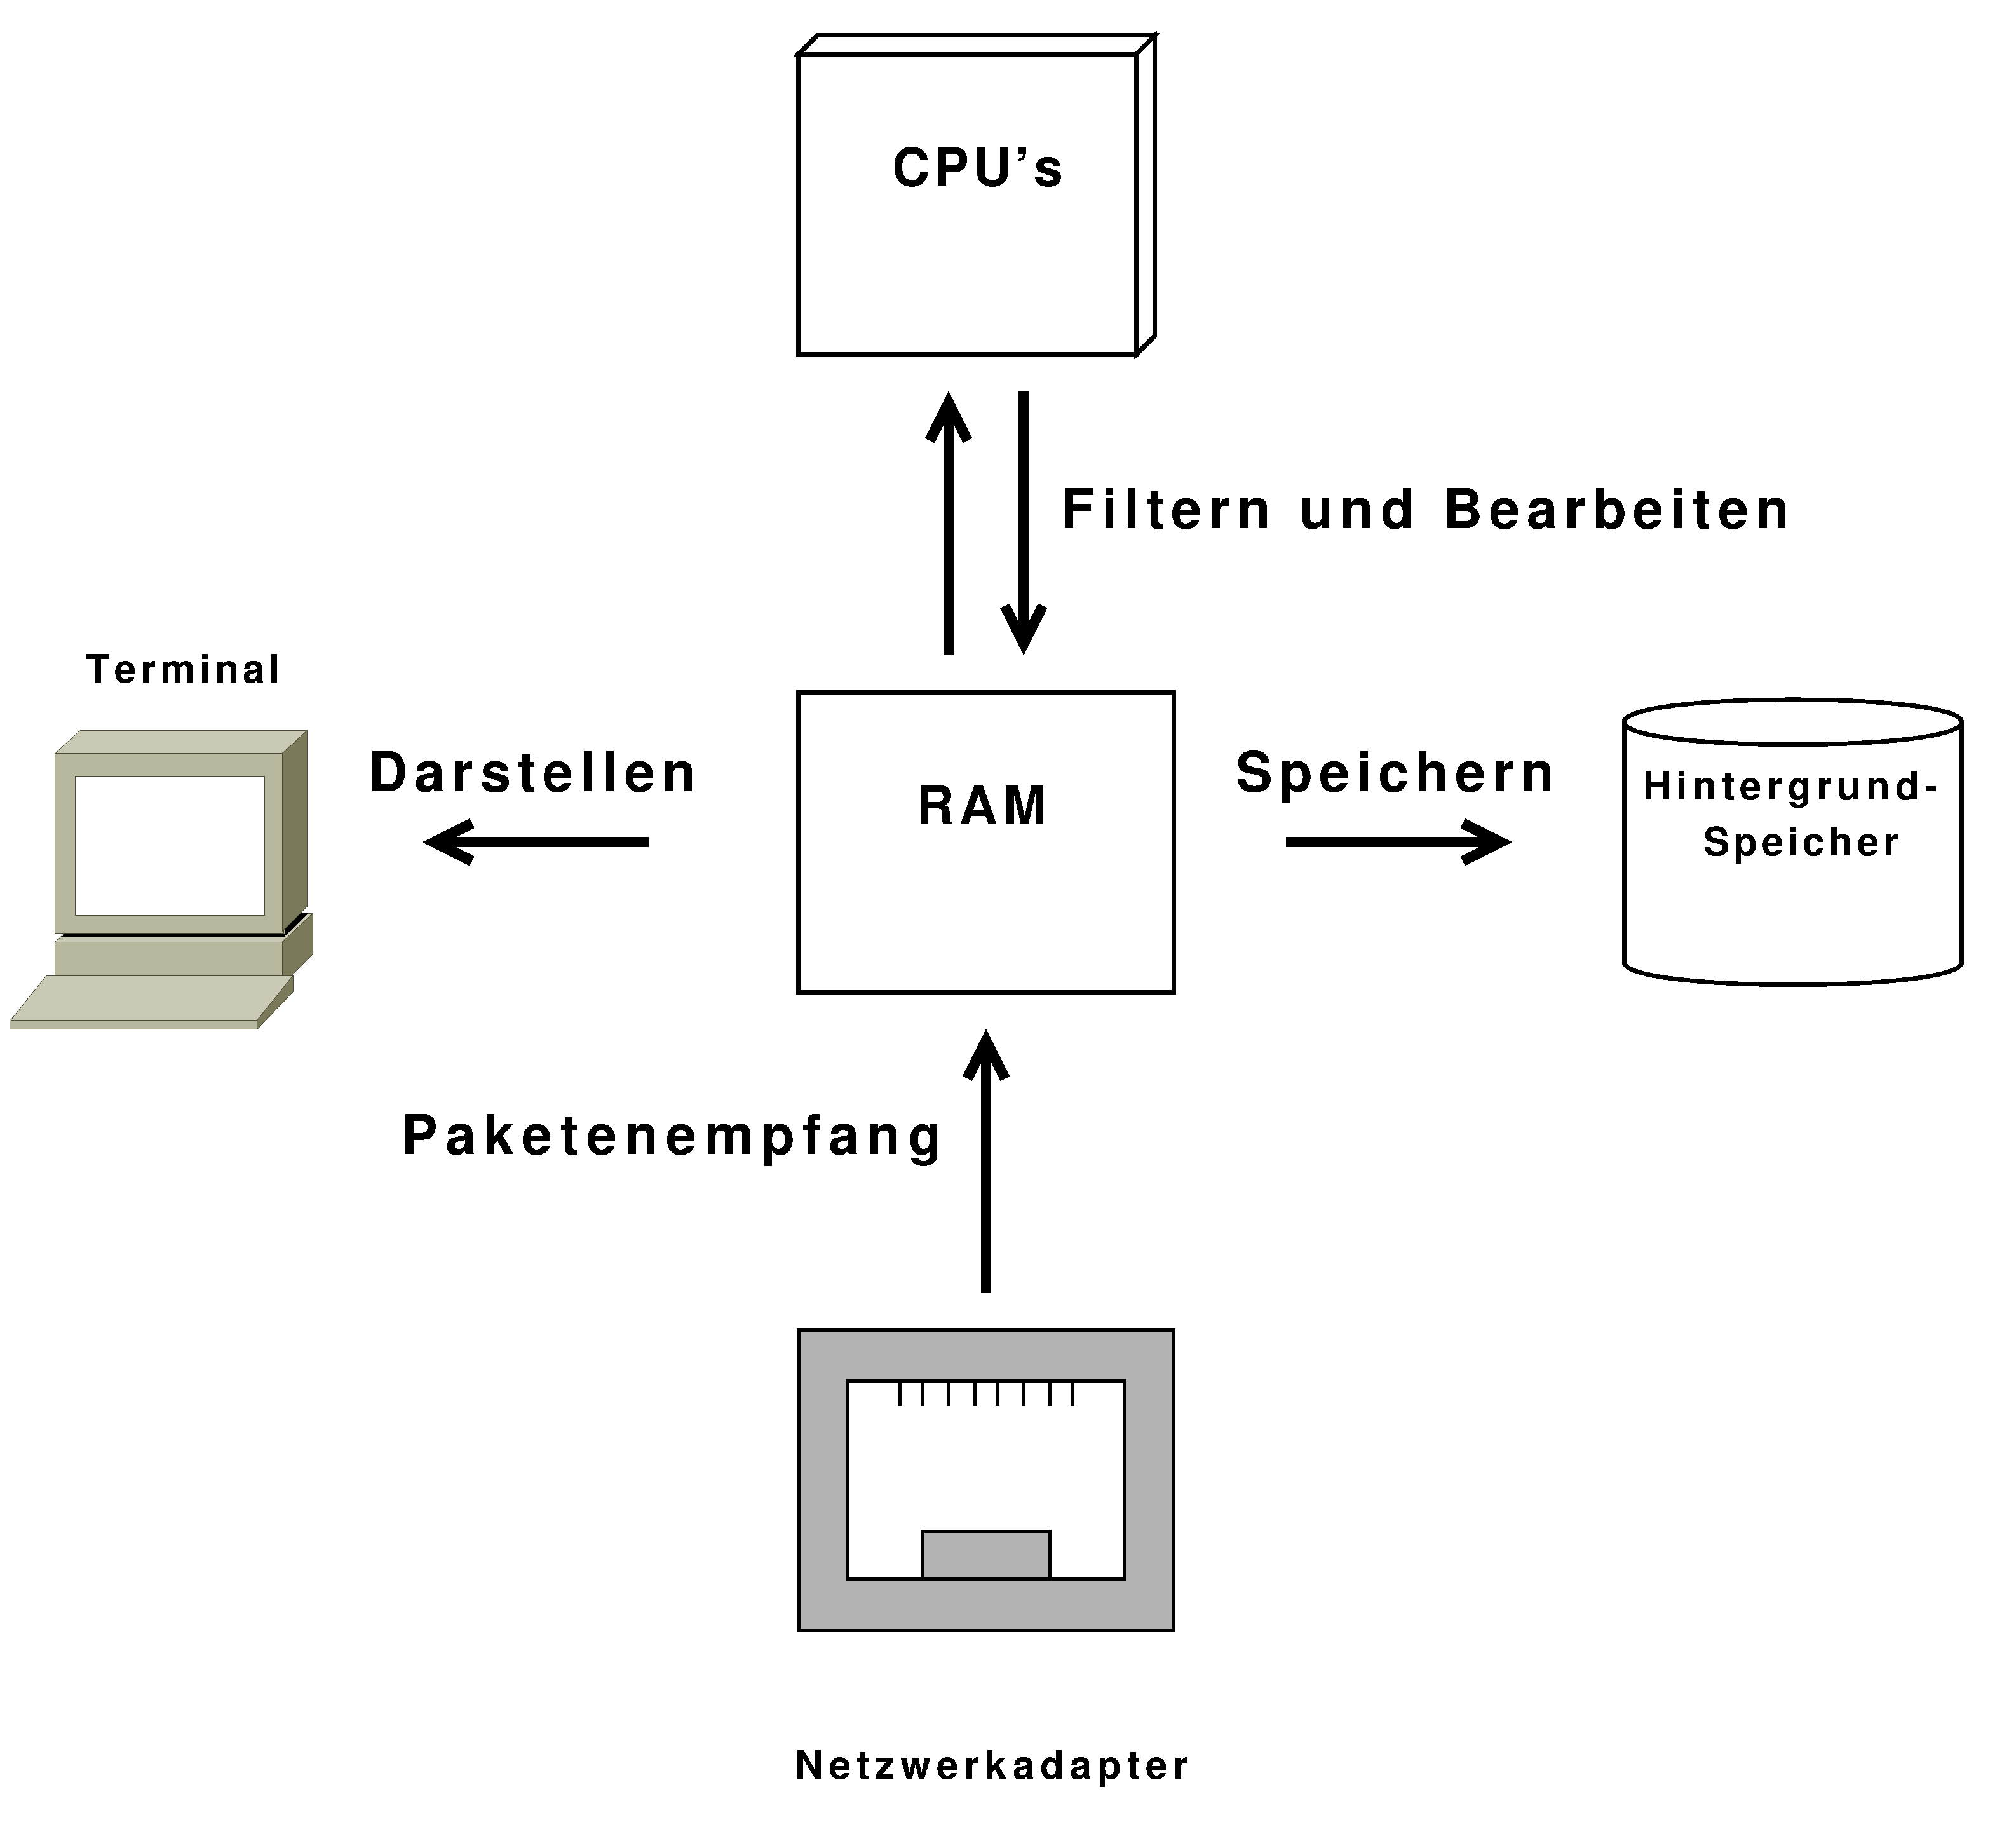
\includegraphics[width=4.0in]{bilder/Capturing}
\caption{Capturing-System}
\label{img:Cap-Sys}
\end{figure}
} 
\subsection{Verwandte Projekte}
\subsubsection*{Zero-Copy BPF Buffers}\label{sec:verw_bpf}
Im Jahr 2007 haben Robert Watson und Christian Peron (Universität Cambridge)
ihre Lösung zur Erhöhung  der Performance von FreeBSD Capturing-Stack
vorgeschlagen und implementiert~\cite{zerocopy}.  Im Rahmen des ``Zero-Copy BPF
Buffers''-Projektes wurde ein neuer Capturing-Stack für das Betriebssystem
FreeBSD entworfen und implementiert.  Im diesem Stack wird das Kopieren der
Paket-Daten in den Userspace, durch Memory-Mapping eliminiert. Dadurch  werden
es keine Kopier-Operationen und keine Systemaufrufe für den Paketzugriff mehr
gebraucht. Da diese Operationen besonders viele CPU Zyklen für ihrer Ausführung
brauchen, verbessert Zero-Copy-Model die Capturing-Performance.\\\\
%
Das Benutzen von Memory-Mapped-Buffers erfordert allerdings ein neues
Konzept für den Zugriff auf Daten. Deshalb wurden im Rahmen des Projektes auch
die Libpcap-Funktionen für den Zugriff auf Pakete im Shared-Buffer angepasst.
Dadurch sind für Capturing-Anwendungen, die auf Libpcap basieren (wie
\emph{tcpdump}), keine Änderungen erforderlich.

%\begin{figure}
%	\begin{center}
%	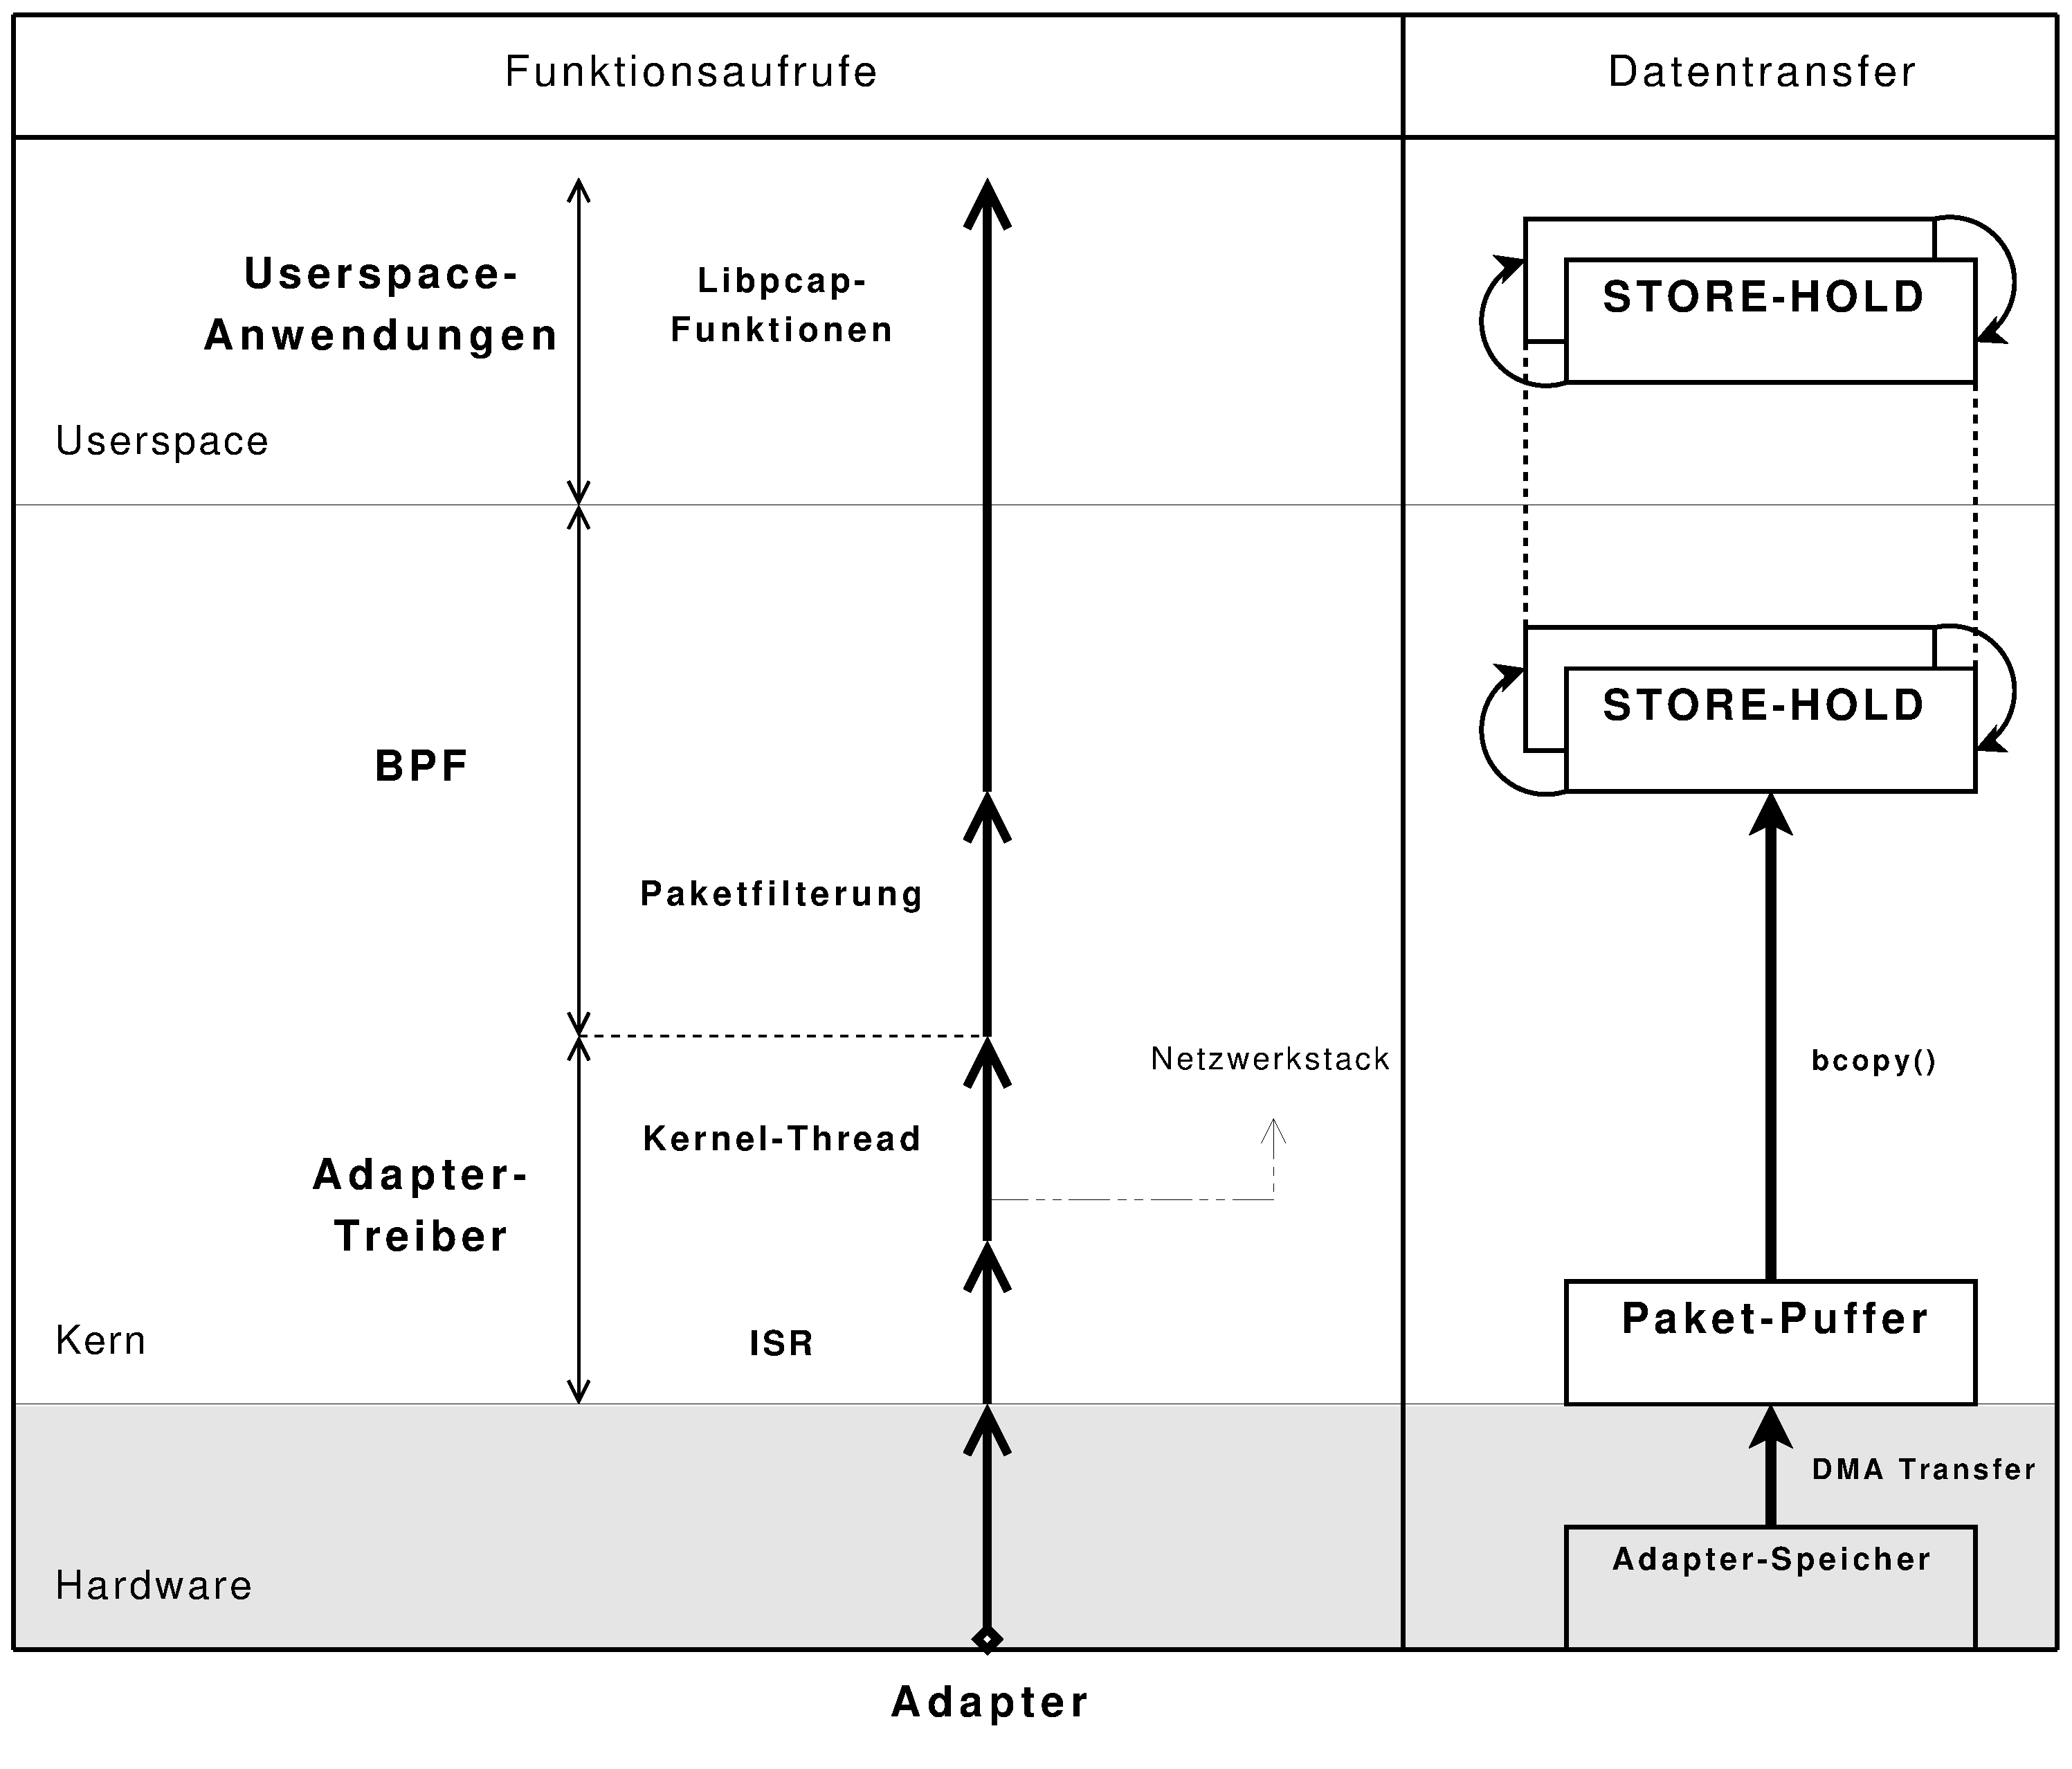
\includegraphics[width=4.9in]{bilder/2copy}
%	\end{center}
%	\caption{Zero-Copy BPF Buffers}
%	\label{img:zc_bpf}
%\end{figure}

\ifthenelse{\boolean{BRIEF}}{}{ 
\subsection{Begriffserklärung}
% \reviewnote{Andi: Warum Definition und Begriffserklärung separat?}

In dieser Diplomarbeit werden oft einige englische Begriffe auftauchen. Sie
haben zwar deutsche Übersetzung, werden aber meistens in ihrer englischen Form
benutzt. Aus diesem Grund gibt es hier eine kurze Begriffserklärung. Auch, weil
der praktische Teil der Diplomarbeit auf einer konkreten Hardware- und
Softwareplattform realisiert wird, sind die Bedeutungen der Begriffe
gezielt dem Kontext der Diplomarbeit angepasst.

\begin{description}
\item[Userspace] ist ein Speicherbereich und Ausführungskontext für
	Useranwendungen.

\item[Kernelspace] ist ein Speicherbereich und Ausführungskontext für den Kern
	des Betriebssystem.

%\reviewnote{Thread is ein Prozess klingt komisch. ggf. Prozess definieren}

\item [Kernel-Thread]
	ist ein Prozess, der vollkommen in Kernelspace ausgeführt wird und keinen 
	direkten Zugriff auf Adressraum eines User-Prozesses hat. Die Kernel-Threads
	werden wie normale Threads in eigenen Threadskontext mit den eigenen Funktions-Stacks
	aber mit einer höhere als bei normalen Threads Prioritäten ausgeführt. 

\item[Interrupt (\emph{Deutsch:} Unterbrechung)] ist ein Ereignis, das den
	Instruktionsfluss auf einer CPU unterbricht und Ausführung einer
	Interrupt-Routine (\emph{Interrupt handler}) auf dieser CPU verursacht.

\item[DMA (\emph{Deutsch:} Speicherdirektzugriff)] bezeichnet eine Art des
	Specherzugriffes, die über Bussystem ohne Beteiligung der CPU realisiert
	ist \cite{dma_wiki}.

\item[Memory-Mapping]  ist eine Funktionalität des Betriebssystem, deren Aufgabe
	es ist, mehrere virtuelle Adressräume auf einen bestimmten physischen
	Speicherraum abzubilden. 

\item[Pointer:] Zeiger

\item[Systemload] ist der prozentuelle Zeitanteil, den CPUs im
	Systemmodus (\emph{protected mode, Ring-0}) verbringen. 

%\reviewnote{Schlecht formuliert:}
\item [Overhead:] Überflüssige Rechenzeiten, Bustransaktionen  und Daten, die
	auf nicht der eigentlichen Aufgabe dienende Prozesse verwendet werden
	müssen.

\item [Descriptor (\emph{Deutsch:} Deskriptor)] ist eine Datenstruktur, die
	zur Beschreibung und Adressierung eines Speichersegmentes dient.
	Descriptor enthält die Anfangsadresse des Segmentes und, eventuell, die
	Länge, die Zugriffsrechte, und andere für das Speichersegment relevante
	Informationen.
\item [Frame] ist Paket auf \emph{link-layer} Ebene. In dieser Diplomarbeit werden
	die Begriffe ``Paket'' und ``Frame'' als Synonyme benutzt. 

\item [NIC (\emph{Network Interfeace Controller})] Netzwerkadapter. In dieser
	Diplomarbeit ist unter diesem Begriff  der Intel Ethernet Gigabit Adapter
	gemeint (siehe \ref{sec:hwsw_voraus}).

\end{description}


\subsection{Struktur der Diplomarbeit}
Das nächste Kapitel \textbf{Grundlagen} präsentiert Hardware- und
Software-Aspekte von Packet-Capturing. Dabei werden zunächst die Funktion der
Hardware vorgestellt, die für die Capturing-Performance relevant ist. Dies
betrifft die Netzwerkkarte, das RAM und den System-Bus.
Unter Software-Aspekten wird der schematisches
Entwurf des Adapter-Treibers und des \emph{Berkley-Packet-Filters} dargestellt.
Außerdem werden in dem Kapitel die Entwurfs-Anforderungen für den neuen
Packet-Capturing-Stack formuliert.\\\\
%
Im Kapitel \textbf{Entwurf} werden Algorithmen zur Verbesserung des FreeBSD
Capturing Stacks vorgestellt. In dem Kapitel werden lediglich logische Lösungen der
Probleme, die bei  Capturing auftauchen, vorgeschlagen. Die Lösung wird zwar
abstrakt dargestellt, basiert dennoch wird auf der konkreten für die Diplomarbeit
vorausgesetzten Hardware.\\\\
%
Im Kapitel \textbf{Implementierung} wird die Struktur der entwickelten Software
vorgestellt. Hierbei werden im Speziellen die Software-Komponenten gezeigt
und kurz erklärt, die für die Umsetzung der im Entwurf vorgestellten
Algorithmen implementiert sind.  \\\\
%
Im Kapitel \textbf{Leistungsbewertung} findet man die Ergebnisse  
des Vergleichs der Performance des FreeBSD-Capturing-Stack im ``generischen''
Fall mit dem neuen, im Rahmen der Diplomarbeit verbesserten, Capturing-Stack. \\\\
%
Im Kapitel \textbf{Schlussfolgerung} wird das wichtigste aus der Diplomarbeit 
in Kurzform dargestellt.  

}
